%NOTE TO SELF:
% Add flowchart of method (and overview)
% Merge section on simulation model and areas of study?
% Merge section on Simulation evaluation and data analysis?
% You can maybe divide the method into two parts: a Hindcast section and a Forecast section

\section{Areas of Study}
	Luzon is the largest island in the Philippines.
	This study analyzed six cities situated in Luzon:
		Angeles,
		Baguio,
		Manila,
		Olongapo,
		Pasay,
		and
		Quezon.
	These cities were chosen because they are all highly-urbanized cities with weather data available from the Integrated Surface Dataset.
	A partial map of Luzon can be seen in Figure \ref{fig:map-of-metro-manila}.

%	This study will be conducted over Metro Manila, Philippines.
%	Metro Manila, formally known as the National Capital Region, is the capital region of the Philippines.
%	The region has a land area of 636 square kilometers	and has a population of 13 million people (\cite{PSA2021}).
%	It is composed of one municipality: Pateros, and sixteen cities:
%		Caloocan,
%		Las Pinas,
%		Makati,
%		Malabon,
%		Mandaluyong,
%		Manila,
%		Marikina,
%		Muntinlupa,
%		Navotas,
%		Paranaque,
%		Pasay,
%		Pasig,
%		Quezon City,
%		San Juan,
%		Taguig, and
%		Valenzuela.
%	A map of Metro Manila is seen in Figure \ref{fig:map-of-metro-manila}.
	
	\begin{figure}
		\centering
		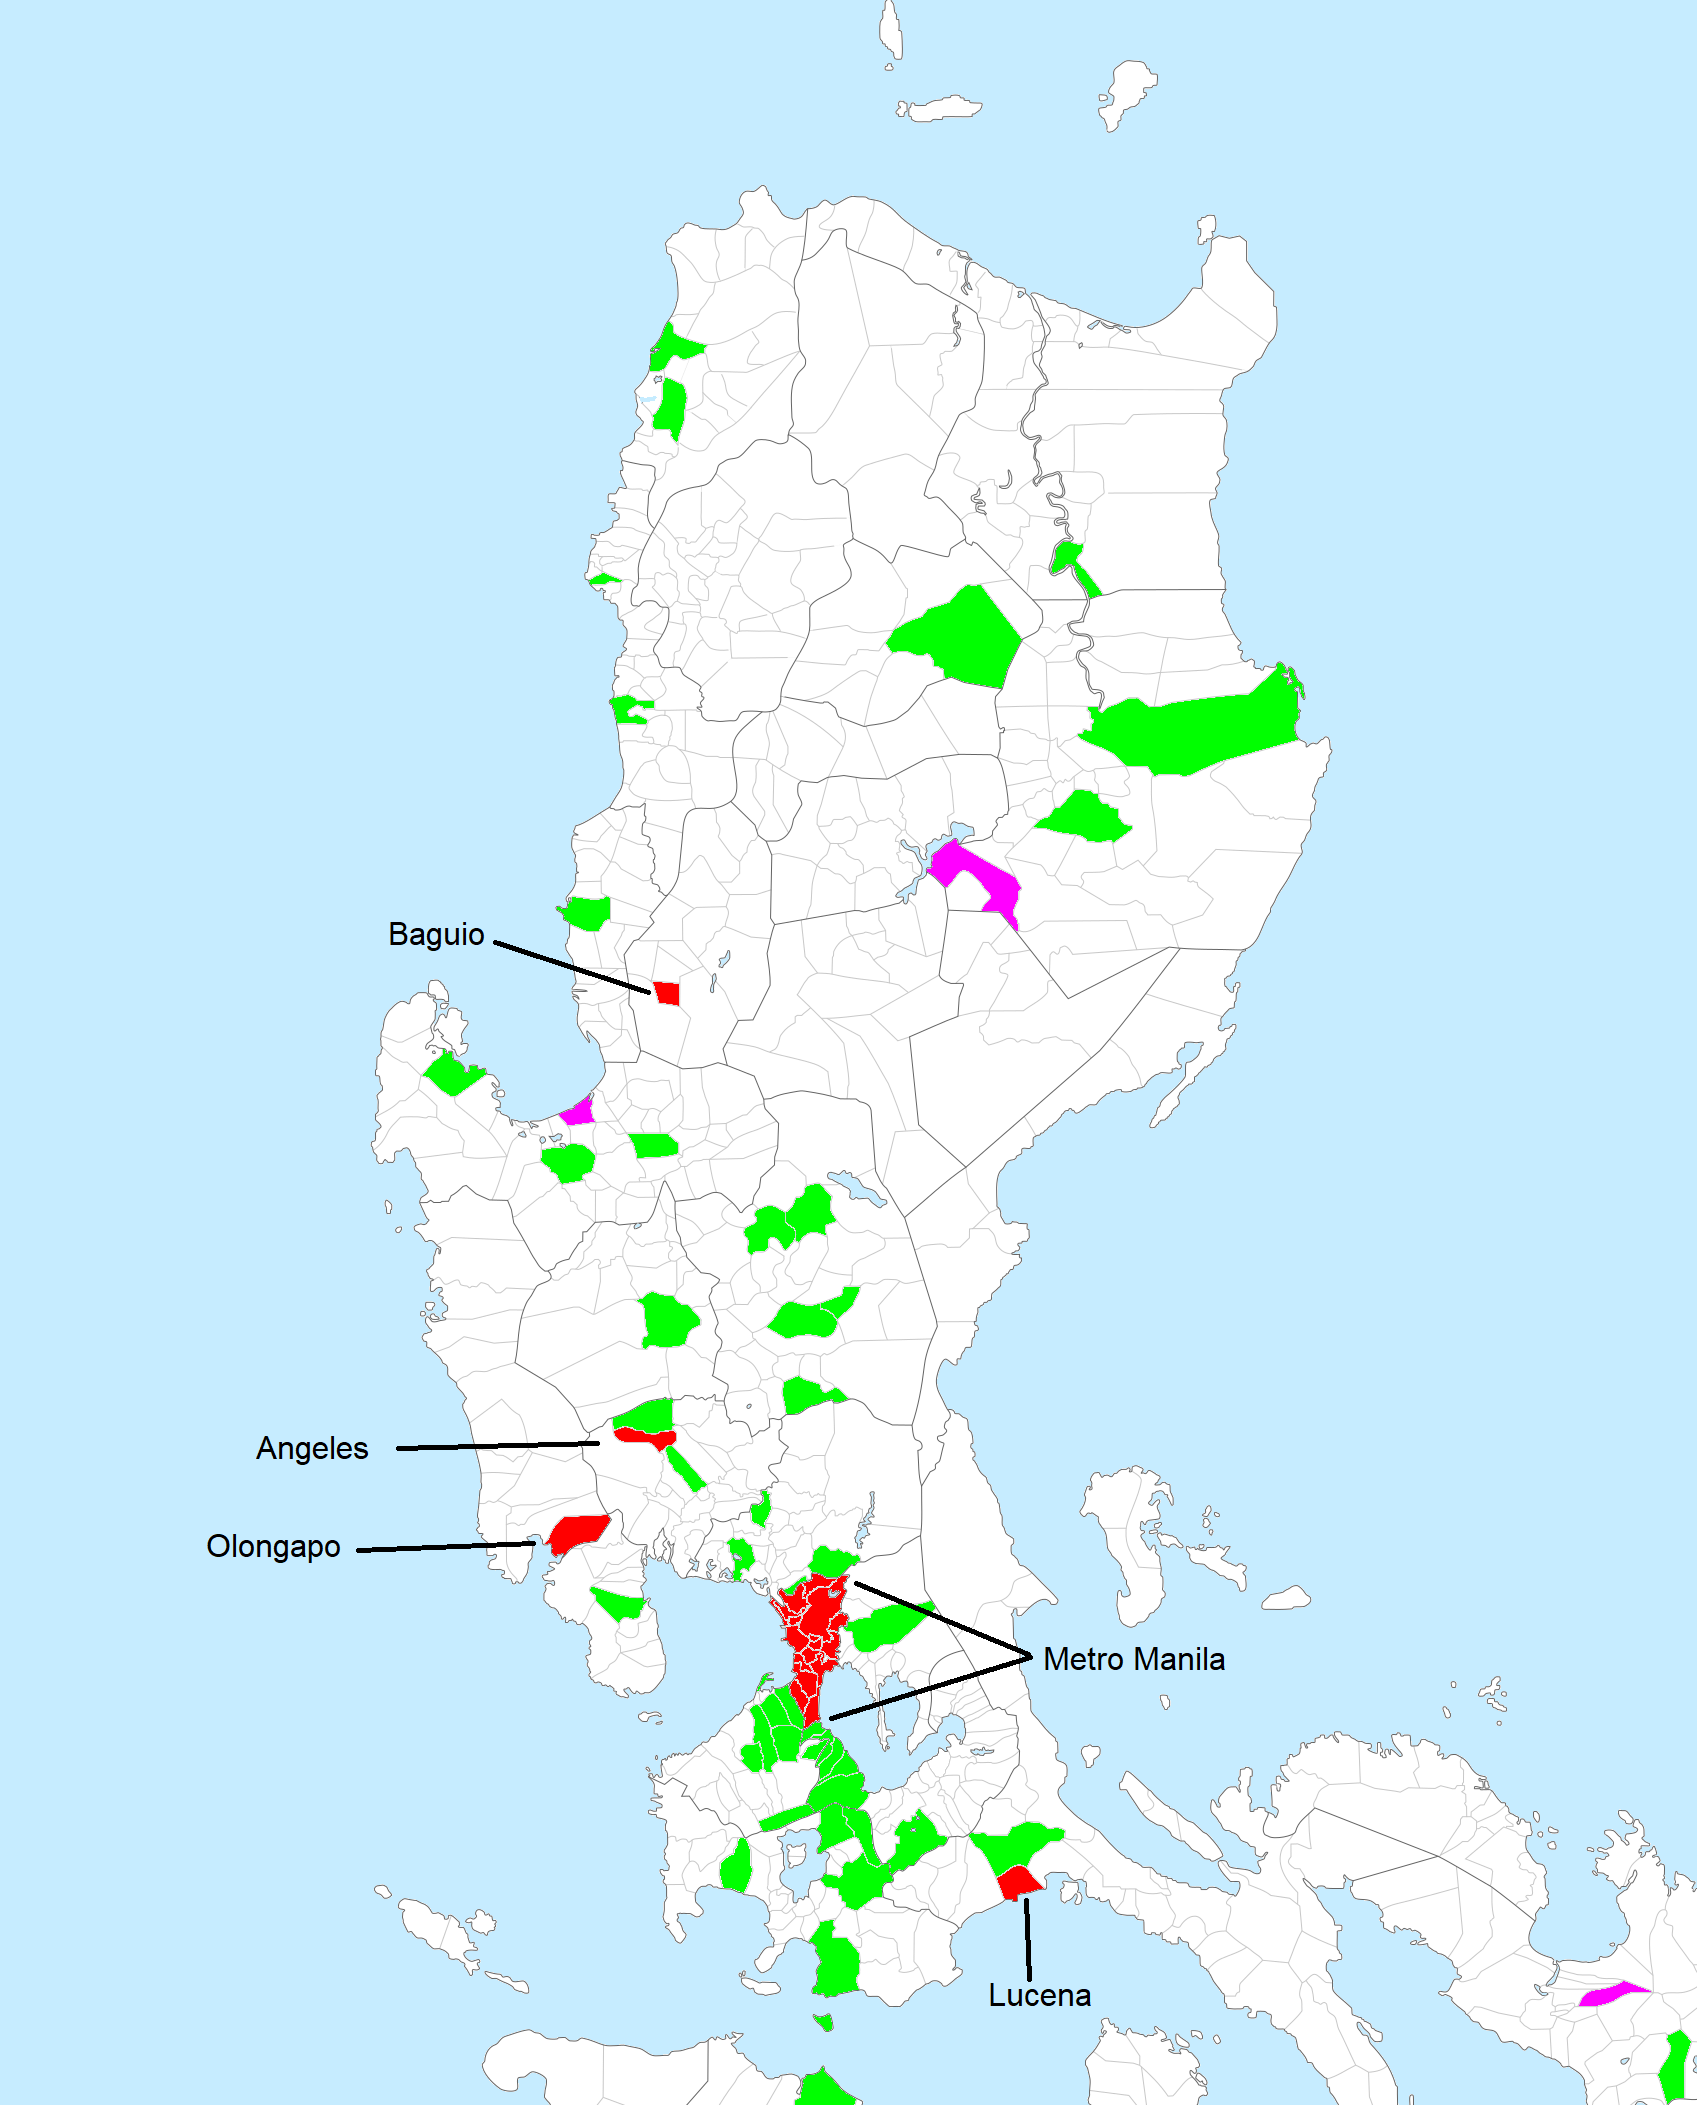
\includegraphics[width=13cm]{map-of-luzon}
		\caption{
			A partial map of Luzon showing its cities and municipalities.
			Highly urbanized cities are highlighted in red,
				Independent Component cities in purple,
				Component cities in green, and
				Municipalities in white.
			Adapted from user Sanglahi86, 	
				\href{https://creativecommons.org/licenses/by-sa/4.0}{CC BY-SA 4.0},
				via \href{https://commons.wikimedia.org/wiki/File:Cities_and_municipalities_of_the_Philippines.png}{Wikimedia Commons}.
		}
		\label{fig:map-of-metro-manila}
	\end{figure}	
		
\section{Simulation Model}
	This study used the latest version of the Regional Climate Model, RegCM5, which is described in detail by \textcite{Giorgi2023}.
	RegCM5 is a limited area model for long-term regional climate simulation.
	It is developed by the Abdus Salam International Centre for Theoretical Physics.
	The previous version, RegCM4, was released in 2012 (\cite{Giorgi2012}).
	
	\begin{table}	
		\caption{Configuration of the RegCM5 physics schemes.}
		\label{tab:physics-schemes}
		\centering
		\begin{tabular}{p{2 in} p{2.75 in}}
			\hline \hline
			Physics scheme & Configuration\\
			\hline
			Atmospheric radiation & Radiation scheme from the Community Climate Model version 3 (\cite{Kiehl1996}) \\
			Land surface model & Community Land Model version 4.5 (\cite{Oleson2013})\\
			Planetary boundary layer & Based on \textcite{Holtslag1990}\\
			Cumulus convection & Based on \textcite{Emanuel1991}\\
			Resolvable scale precipitation & Subgrid explicit moisture scheme (SUBEX) (\cite{Pal2000})\\
			\hline
		\end{tabular}		
	\end{table}

	A figure of the domain can be seen in Fig X.
	This study conducted simulations over two periods: a present period and a future period.
	For the present period, this study conducted simulations of Luzon over a four-year period, starting from 2014, January 2 up to 2018, January 1.
	The first year was considered as spin-up time and was ignored.
	Thus, only the three-year simulation period from 2015, January 1 to 2018, January 1 was considered for the data analysis.
	The simulation is set to output the results every 3 hours.
	The results of this simulation was compared to real meteorological data in order to determine the performance of the simulation.
	After the simulation has been evaluated to perform well, the second simulation was run.
	The second simulation was conducted from 2026 to 2030 to study the future.
	
	Table \ref{tab:physics-schemes} shows the physics schemes used in the study.
	These schemes, with the exception of the land surface model, was used because they are the default schemes. 
	For the land surface model, the Community Land Model version 4.5 was chosen over the default, the Biosphere-Atmosphere Transfer Scheme. 
	The Community Land Model has a model for urban energy balance and climate, which the default model lacks.
	
\section{Simulation Evaluation}
	To determine the performance of the simulation, an evaluation was performed. The evaluation procedure was adapted from \textcite{Bilang2022}.
	The results of the simulation was compared to real data from the Integrated Surface Database (ISD).
	The ISD is maintained by the United States National Oceanic and Atmospheric Administration, and is readily available on their website 
		(\url{https://www.ncei.noaa.gov/products/land-based-station/integrated-surface-database}).
	Data points missing from the data set were handled by replacing them with the mean of the data.
	The areas of study as well as their corresponding stations to be used in the evaluation are listed in Table \ref{tab:isd-stations}.

	\begin{table}	
		\caption{Areas of study and their corresponding stations in the Integrated Surface Dataset (ISD).}
		\label{tab:isd-stations}
		\centering
		\begin{tabular}{ll}
			\hline \hline
			Area of Study             & ISD Station Name                       \\
			\hline
			Angeles, Pampanga         & Clark International Airport        \\
			Baguio, Benguet           & Baguio                             \\
			Manila, Metro Manila      & Manila                             \\
			Olongapo, Zambales        & Cubi Point                         \\
			Pasay, Metro Manila      & Ninoy Aquino International Airport \\
			Quezon City, Metro Manila & Science Garden \\                   
			\hline
		\end{tabular}	
	\end{table}

	Four performance statistics were computed using equations \ref{eq:mean-bias} to \ref{eq:y-bar},
		where $y_i$ is the modeled value, $y_{i,\text{obs}}$ is the observed value, and $N$ is the number of data points (\cite{Bilang2022}).
	The mean bias (MB) is a measure of the model to overestimate or underestimate a variable (\cite{Carbonell2013}), and is calculated by
	\begin{equation}
		\text{MB} =
			\frac{1}{N}
			\sum_{i=1}^{N}
			(y_i - y_{i,\text{obs}}).
			\label{eq:mean-bias}
	\end{equation}
	The mean absolute error (MAE) is used to measure the closeness of the modeled and observed values (\cite{Arasa2016}).
	It is calculated by
	\begin{equation}
		\text{MAE} =
			\frac{1}{N}
			\sum_{i=1}^{N} 
			|y_i - y_{i,\text{obs}}|. \label{eq:mean-absolute-error}
	\end{equation}
	The root mean square error (RMSE) is similar to the MAE but more sensitive to large errors due to the squared term (\cite{Carbonell2013}).
	It is calculated by
	\begin{equation}
		\text{RMSE} =
		\sqrt{
			\frac{
				\sum_{i=1}^{N}
				(y_i - y_{i,\text{obs}}) ^ 2
			}{N}
		}.
		\label{eq:root-mean-square-error}
	\end{equation}
	Lastly, the index of agreement (IOA), introduced by \textcite{Willmott1980}, shows how an error-free model predicts a variable.
	The index ranges between \num{0} and \num{1},
		with a value of \num{0} meaning no agreement between the model and observed data,
		and a value of \num{1} meaning a perfect match. 
	It is computed as
	\begin{equation}
		\text{IOA} =
			1 - 
			\frac{
				\sum_{i=1}^{N}
				(y_i - y_{i,\text{obs}}) ^ 2
			}{
				\sum_{i=1}^{N} (
					|y_i - \bar{y}| +
					|y_{i,\text{obs}} - \bar{y}|
				)^2
			},
			\label{eq:index-of-agreement}
	\end{equation}
	where
	\begin{equation}
		\bar{y} = 
			\frac{1}{N}
			\sum_{i=1}^{N} y_{i,\text{obs}}.
			\label{eq:y-bar}
	\end{equation}
	Before computing the statistics, the model values were first rounded to the nearest tenth in order to match the accuracy of the observed values from the ISD.
	The threshold for these values to determine if the model is performing well are given in Table \ref{tab:performance-statistics-threshold}, as adapted from \textcite{Bilang2022}.

	\begin{table}	
		\caption{Recommended values of statistical tests for near-surface air temperature.}
		\label{tab:performance-statistics-threshold}
		\centering
		\begin{tabular}{l l}
			\hline \hline
			Statistical parameter & Criteria\\
			\hline
			MB & $\leq \pm \qty{2.0}{\degreeCelsius}$ \\
			RMSE & $\leq \qty{3.5}{\degreeCelsius}$\\
			MAE & $\leq \pm \qty{2.0}{\degreeCelsius}$\\
			IOA	& $\geq \num{0.8}$\\
			\hline
		\end{tabular}		
	\end{table}

\section{Data Graphing and Analysis}
	The results of the simulations were graphed.
	Data for the near-surface air temperature were graphed as a function of time.
	This is to visually see the trend of the air temperature as time progresses.
	For the simulation of the present time, the graph of the simulation results will be overlayed on the graph of the observed data from the ISD.
	This is to visually compare the performance of the simulation with actual data.
	
	The results of the simulations were also statistically analyzed.
	Descriptive statistics for the near-surface air temperature, such as the mean, maximum, and minimum temperature, were be computed.
	A linear regression was applied to see the trend at which temperature changes as time progresses.